\chapter{Results \label{Chapter-Results}}

\section{PPG Preprocessing through the VAE}

One of the preprocessing techniques used to "downsample" the PPG signal was the Variational Autoencoder (VAE), whose encoder could be used to transform each 256Hz second into a 1Hz value of 8 dimensions. We tried two versions: The first got a 1-second input and had to reconstruct the exact second. The other one go a 2-second window around the second it should reconstruct. Figure \ref{fig:vaereconstruction} shows the example reconstructions of the two variations and Figure \ref{fig:vaeloss} plots the reconstruction losses over the epochs. As the 5s VAE had a lower loss, we used its encoder for the VAE preprocessing option.

\begin{figure}[h]
    \centering
    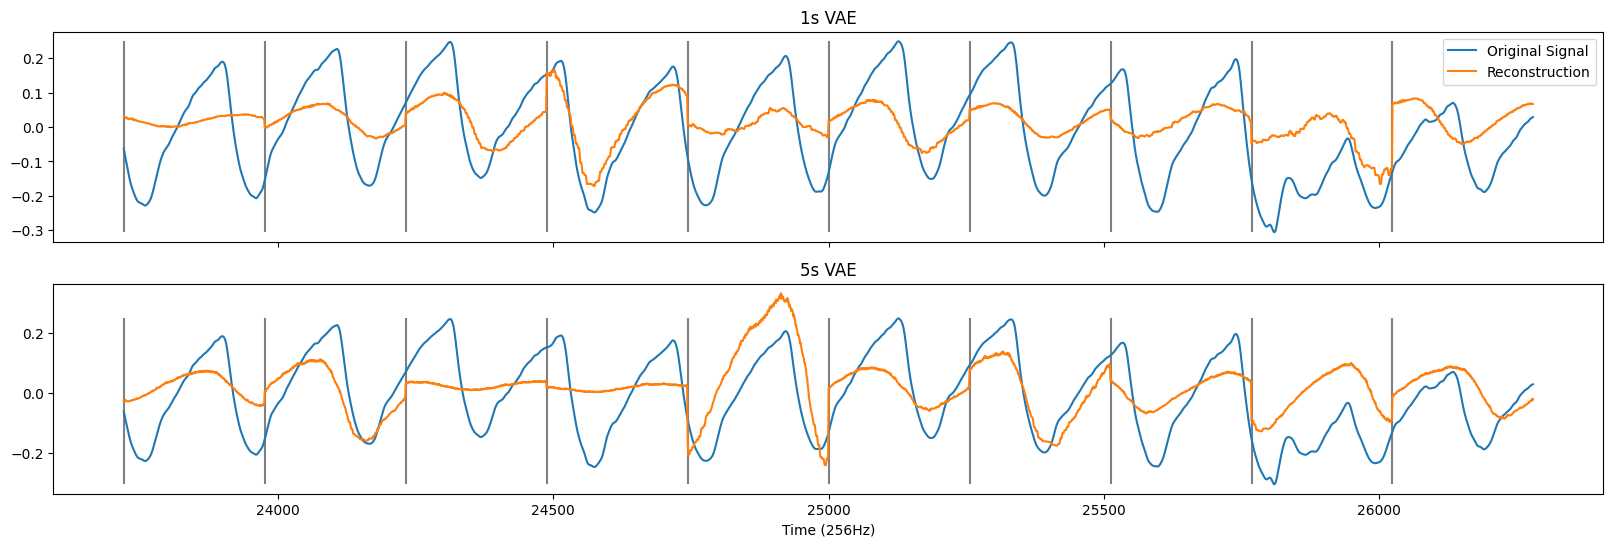
\includegraphics[width=\textwidth]{images/VaeReconstruction}
    \caption{Example difference in reconstructions of the 1s and 5s VAE for the same signal. Each second has 256 values, which are reduced to only 8 values.}
    \label{fig:vaereconstruction}
\end{figure}

\begin{figure}
    \centering
    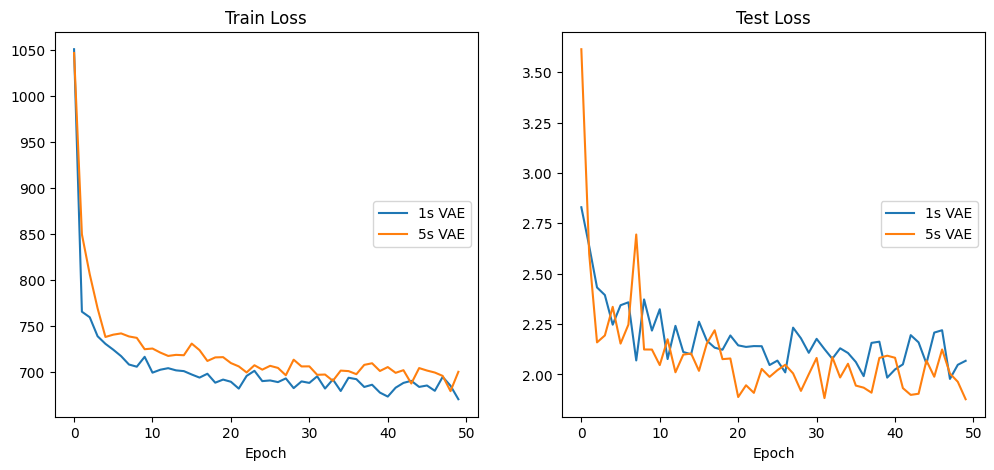
\includegraphics[width=\textwidth]{images/VaeLoss}
    \caption{Train and test loss of both VAEs. Although the 1s VAE had a lower train loss, the 5s performed better on the test set, which could be a sign of better generalization.}
    \label{fig:vaeloss}
\end{figure}

\section{Preprocessing impact on performance}

Figure \ref{fig:preprocessingresults} shows the recall, precision, and F1-score for the SDB detection model with the different preprocessing techniques. While neither the statistical nor the VAE preprocessing approach reached the same performance as the in-model approach, using both statistical and VAE preprocessing together did reach a similar performance. As both these values would only be needed to be calculated once before the training and not during each epoch, which the in-model approach did, training time got reduced significantly by a factor of 3. This can be seen in Table \ref{tab:preprocessing-times}.

\begin{figure}
    \centering
    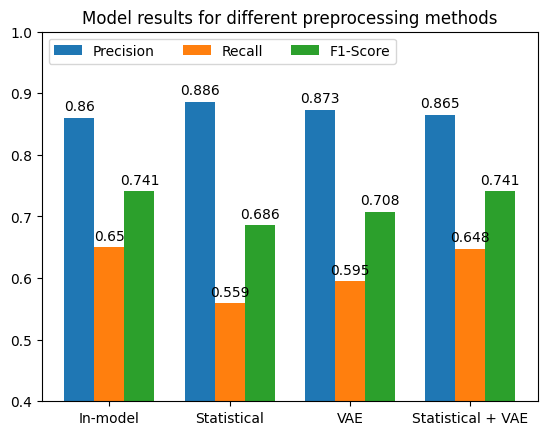
\includegraphics[width=0.6\textwidth]{images/PreprocessingResults}
    \caption{Precision, recall, and F1-score of the SDB detection model with different preprocessing techniques. Although the precision didn't change much, the recall and therefore the F1-score dropped significantly, when using the statistical or VAE preprocessing only.
    Important to note is that these results came from experiments with the ground-truth hypnogram, which is not the final model, as the final model uses the PPG-predicted hypnogram.}
    \label{fig:preprocessingresults}
\end{figure}

\renewcommand{\arraystretch}{1.5}
\begin{table}
    \centering
    \begin{tabular}{ l c c }
        Method & Training time & Testing time \\
        \hline
        In-model & 145min & 34min \\
        Statistical & 46min & 12min \\
        VAE & 47min & 12min \\
        Stat. + VAE & 50min & 12min \\
    \end{tabular}
    \caption{SDB detection model training and testing times in minutes. The in-model approach took roughly three times as long. \label{tab:preprocessing-times}}
\end{table}

\section{SDB Detection Model}

\subsection*{Event-level performance}

Figure \ref{fig:event-metrics} shows the recall, precision, and F1-score over each threshold for the main SDB detection model, which uses the PPG-predicted hypnogram, the PPG itself with the in-model technique, and the SpO2. The Figure also shows a version of the model without the SpO2 signal, which means it relies solely on the PPG data. As can be seen, omitting the SpO2 signal has a significant impact on the performance, as the peak F1-score drops from 69.7\% to 61.6\%. The threshold for the best performance was determined to be 0.25.

\begin{figure}
    \centering
    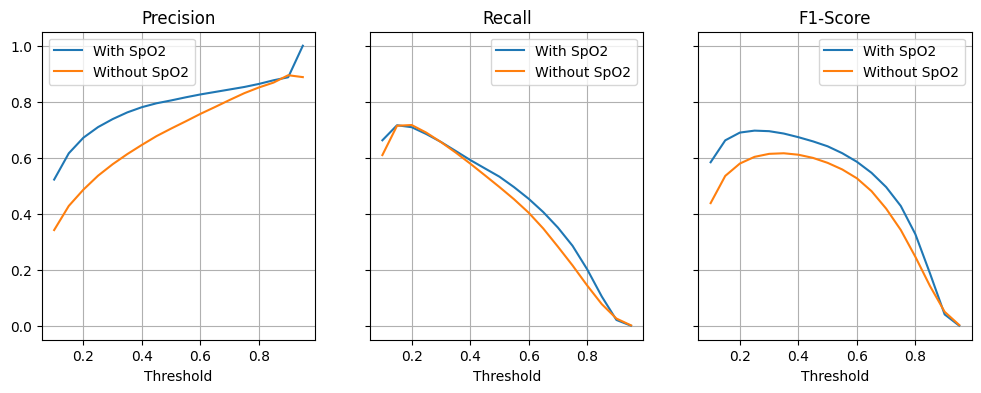
\includegraphics[width=\textwidth]{images/DetectionModelEventMetrics}
    \caption{Comparison of the event-level metrics of the SDB detection model with and without SpO2. The model with SpO2 reached a peak F1-score of 69.7\% at a threshold of 0.25, while the one without SpO2 only reached a peak F1-score of 61.6\% at a threshold of 0.35.}
    \label{fig:event-metrics}
\end{figure}

Test and training losses together with the peak F1-score over the epochs are displayed in Figure \ref{fig:event-epoch-losses}. While the version without SpO2 seems to train slightly more stable, learning convergences much slower than the one with SpO2, which reaches the area of the final peak F1-score in the first few epochs.

\begin{figure}
    \centering
    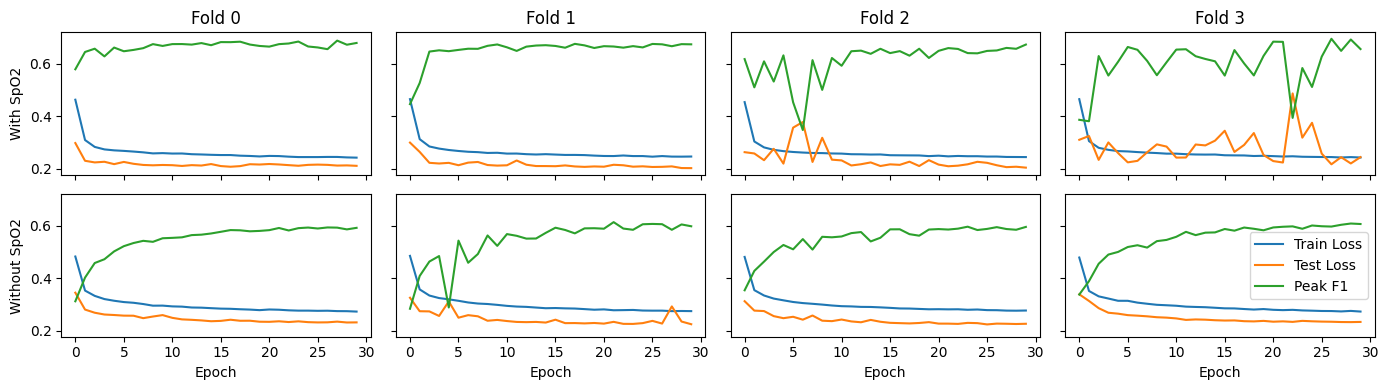
\includegraphics[width=\textwidth]{images/DetectionModelEpochLosses}
    \caption{Losses and peak F1-score by epoch for every fold.}
    \label{fig:event-epoch-losses}
\end{figure}

We show our final event-level metrics together with a comparison to other studies in Table \ref{tab:final-metrics}.

\renewcommand{\arraystretch}{1.5}
\begin{table}
    \centering
    \begin{tabular}{ l l c c c }
        Model & Signals & Prec. & Rec. & F1\\
        \hline
        \cite{olsen2020robust}* & ECG & 73.4\% & 70.9\% & 72.1\% \\
        \cite{xie2023use}* & ECG, RE & 56.5\% & 77.4\% & 70.8\% \\
        \cite{xie2024multi} & ECG, RE & 63.3\% & 63.0\% & 63.1\% \\
        \cite{li2023deep}** & Airflow, EEG & 87.3\% & 83.7\% & 85.7\% \\
        \cite{yook2024deep}** & Airflow, SpO2 & 93.0\% & 91.0\% & 93.0\% \\
        \cite{lazazzera2020detection}** & PPG, SpO2 & - & 76.9\% & - \\
        Ours & PPG, SpO2 & 70.94\% & 68.46\% & 69.68\% \\
    \end{tabular}
    \caption{Result comparison between other work and our SDB detection model. Models that use the airflow signal achieve the best results. *Studies that use the ground-truth, PSG-computed sleep stages. **Studies that classify 60- or 10-second long epochs instead of events, as our event scoring metric does. \label{tab:final-metrics}}
\end{table}

With the threshold of 0.25, we can analyse the performance based on the event class and sleep stage. Table \ref{tab:event-class-distribution} shows the distribution of event classes in the dataset and the models detection rate. The dataset is highly imbalanced, with 2/3 of all events being hypopneas. Still, the model was best in detecting mixed apneas, with a near 90\% detection rate, while hypopneas were only detected about 2/3 of the time.

\renewcommand{\arraystretch}{1.5}
\begin{table}
    \centering
    \begin{tabular}{ l p{2cm} p{2cm} p{2cm} p{2cm} }
        & Obstructive \newline Apnea & Mixed \newline Apnea & Central \newline Apnea & Hypopnea \\
        \hline
        Total (N) & 61161 & 4811 & 15240 & 162536 \\
        \% of all & 25.1\% & 2.0\% & 6.3\%  &  66.7\% \\
        \hline
        Found (N) & 43243 & 4299 & 12486 & 111826 \\
        \% found & 70.7\% & 89.4\% & 81.9\% & 68.8\% \\
    \end{tabular}
    \caption{Distribution of event classes in the full dataset and how many of the different classes were detected by our model. Although the dataset is greatly inbalanced to hypopneas (2/3 of all) and against mixed apneas (only 2\%), the detection rates greater for apneas than for hypopneas. \label{tab:event-class-distribution}}
\end{table}

In appendix \todo{ref} we show and discuss the results per sleep stage and the length of the predicted events.

\subsection*{AHI-level performance}

Figure \ref{fig:ahi-plots} shows the scatter plots for the predicted and true AHI values of both versions of the model. To assess agreement, Figure \ref{fig:bland-altman-plots} displays the corresponding Bland-Altman plots. Both plots show a bias towards predicting higher AHIs for the model without SpO2, while the one with PPG and SpO2 shows lower deviation and near to no bias. We also got a lower RMSE of 7.6 instead of 11.8 when using SpO2.
For the model with SpO2 we achieved a Spearman rank correlation of 0.917 and an intra-class correlation of  0.91.
All AHI-level metrics and a comparison to other work can be found in Table \ref{tab:ahi-level-metrics}.

\begin{figure}
    \centering
    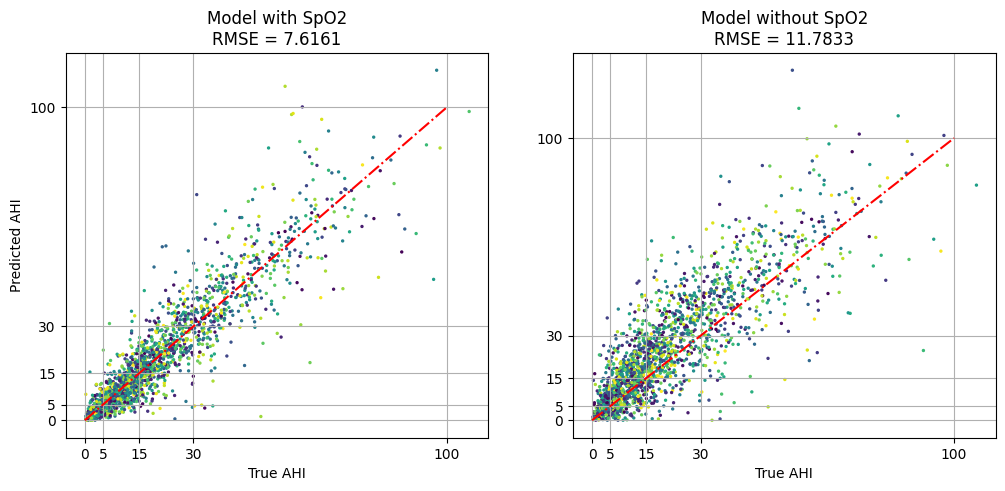
\includegraphics[width=\textwidth]{images/AhiPlots}
    \caption{Preedicted AHI plotted against the ground-truth AHI. The left plot shows the model with SpO2 and PPG. The right one shows the result of using only PPG as input. The red line is the identity line. The grid shows the differen AHI severity class boundaries.}
    \label{fig:ahi-plots}
\end{figure}

\begin{figure}
    \centering
    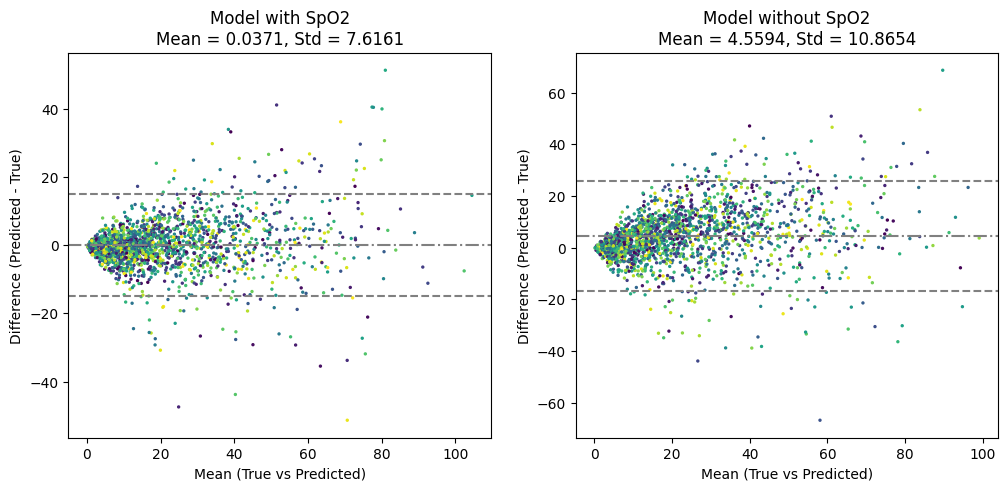
\includegraphics[width=\textwidth]{images/BlandAltmanPlots}
    \caption{Bland-Altman plots for the true and predicted AHI values. The left plot shows the model with SpO2 and PPG. The right one shows the result of using only PPG as input. The grey line is the mean difference and the grey, dashed lines are levels of agreement, computed as 1.96 times the standard deviation of the differences.}
    \label{fig:bland-altman-plots}
\end{figure}

\renewcommand{\arraystretch}{1.5}
\begin{table}
    \centering
    \begin{tabular}{ l p{1cm} p{2.5cm} p{1cm} p{1cm} p{1.5cm} }
        Model & $\rho$ & ICC, 95\%CI & RMSE & Bias & SD error \\
        \hline
        PPG + SpO2 & \textbf{0.917} & \textbf{0.91} [0.90, 0.92] & \textbf{7.62} & \textbf{0.04} & \textbf{7.62} \\
        PPG only   & 0.842 & 0.81 [0.73, 0.86] & 11.8 & 4.56 & 10.8 \\
        \hline
        \cite{fonseca2024estimating}, MESA & 0.87 & 0.88 [0.86, 0.90] & 9.67 & -0.58 & 9.66 \\
        \cite{fonseca2024estimating}, All datasets & 0.89 & 0.91 [0.89, 0.92] & 8.88 & -0.85 & 8.84 \\
    \end{tabular}
    \caption{AHI-level metrics for our work with and without SpO2 compared to results from Fonseca et al. Both Spearman's $\rho$ and the ICC are statistically significant with $p < 0.0001$. \label{tab:ahi-level-metrics}}
\end{table}

\subsection*{Severity-class-level performance}

Figure \ref{fig:severity-class-level-confusion-matrices} shows the confusion matrices for the predicted severity classes using the hard thresholds and the NBL version. Although a strong focus on the true prediction diagonal can be seen in both models, the bias towards predicting higher severity classes for the PPG only model is still visible.

\begin{figure}
      \begin{subfigure}{\textwidth}
          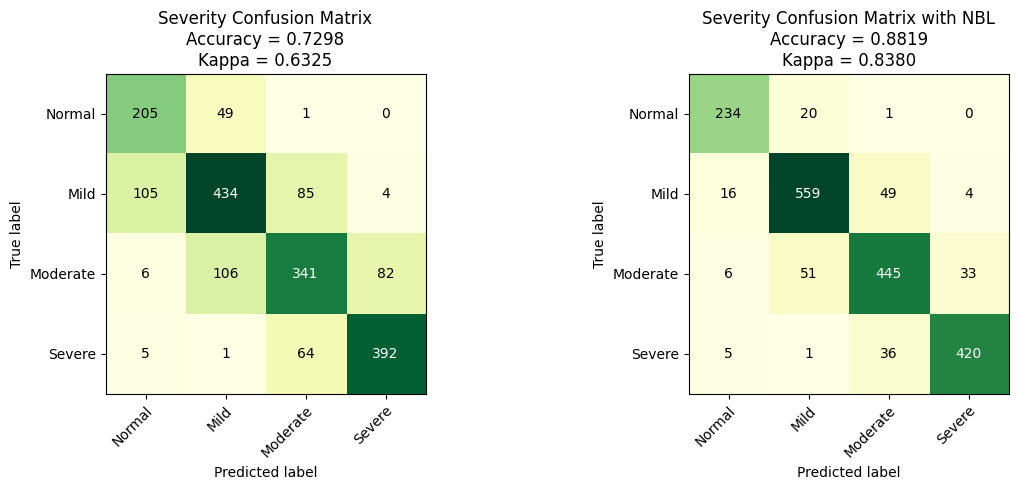
\includegraphics[width=\textwidth]{images/SevClassConfMatrix}
          \caption{Model with SpO2 and PPG}
      \end{subfigure}
      \begin{subfigure}{\textwidth}
          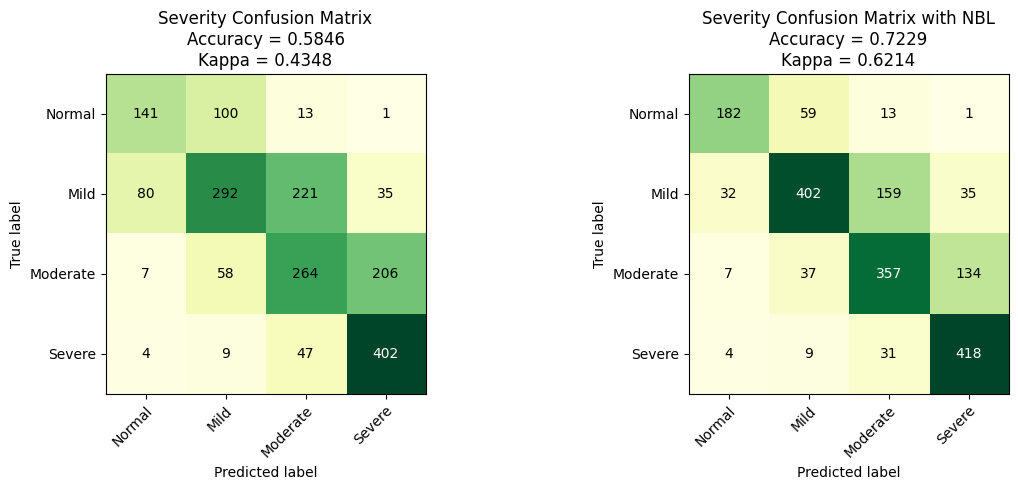
\includegraphics[width=\textwidth]{images/SevClassConfMatrixNoSpO2}
          \caption{Model with PPG only}
      \end{subfigure}
    \caption{Confusion matrices for the predicted and true severity classes with and without NBL and for both models. (a) shows the model with SpO2 and PPG, while (b) shows the model with PPG only.}
    \label{fig:severity-class-level-confusion-matrices}
\end{figure}

We show the models discrimination ability in Table \ref{tab:severity-class-level-metrics}, where we show binarized confusion matric results for no SDB vs SDB, mild vs moderate SDB, and moderate vs severe SDB. As before, the model with access to SpO2 performed better and NBL increased results. Most PPG + SpO2 model metrics exceed 90\% while the PPG only model struggles especially with specificity and NPV. Likelihood ratios are also shown, achieving values of $\geq 4$ and $\leq 0.2$ for positive and negative likelihood ratios respectively in most cases, showing good diagnostic performance.

\renewcommand{\arraystretch}{1.5}
\begin{table}
    \centering
    \begin{tabular}{ p{1.5cm} p{2cm} p{1cm} p{1cm} p{1cm} p{1cm} p{1cm} p{1cm} p{1cm} }
        Min. \newline Sev. & N $\geq$ thr \newline (\% $\geq$ thr)  & Acc. & Sens. & Spec. & PPV & NPV & LR+ & LR- \\
        \hline
        \hline
        \multicolumn{5}{c}{PPG + SpO2} \\
        \hline
        Mild & 1625 (86\%) & 0.912 & 0.929 & 0.804 & 0.968 & 0.639 & 4.736 & 0.089 \\
        Moderate & 997 (53\%) & 0.889 & 0.882 & 0.898 & 0.907 & 0.870 & 8.650 & 0.132 \\
        Severe & 462 (25\%) & 0.917 & 0.848 & 0.939 & 0.820 & 0.950 & 13.990 & 0.161 \\
        \hline
        \multicolumn{5}{c}{PPG + SpO2 (NBL)} \\
        \hline
        Mild & 1625 (86\%) & \textbf{0.974} & \textbf{0.983} & 0.918 & \textbf{0.987} & 0.897 & 11.941 & \textbf{0.018} \\
        Moderate & 997 (53\%) & 0.938 & 0.937 & 0.939 & 0.945 & 0.929 & 15.319 & 0.067 \\
        Severe & 462 (25\%) & 0.958 & 0.909 & \textbf{0.974} & 0.919 & \textbf{0.970} & \textbf{34.840} & 0.093 \\
        \hline
        \hline
        \multicolumn{5}{c}{PPG only} \\
        \hline
        Mild & 1625 (86\%) & 0.891 & 0.944 & 0.553 & 0.931 & 0.608 & 2.112 & 0.101 \\
        Moderate & 997 (53\%) & 0.815 & 0.922 & 0.694 & 0.773 & 0.887 & 3.015 & 0.113 \\
        Severe & 462 (25\%) & 0.839 & 0.870 & 0.829 & 0.624 & 0.951 & 5.099 & 0.157 \\
        \hline
        \multicolumn{5}{c}{PPG only (NBL)} \\
        \hline
        Mild & 1625 (86\%) & 0.938 & 0.974 & 0.714 & 0.956 & 0.809 & 3.401 & 0.037 \\
        Moderate & 997 (53\%) & 0.859 & 0.943 & 0.764 & 0.819 & 0.922 & 4.002 & 0.075 \\
        Severe & 462 (25\%) & 0.886 & 0.905 & 0.880 & 0.711 & 0.966 & 7.547 & 0.108 \\
    \end{tabular}
    \caption{Diagnostic performance of our models. The best values all come from the PPG + SpO2 model with NBL. \label{tab:severity-class-level-metrics}}
\end{table}

\section{Importance of correct Sleep Stages}

To assess the importance of the correct sleep stage prediction, we trained a model with the ground-truth hypnogram, the PPG-generated hypnogram, and finally without any sleep stage information, letting the model only rely on PPG and SpO2. Figure \ref{fig:sleep-stage-importance} shows the event-level metrics for each of these experiments. With the exception of the recall for lower thresholds, the models performance reduces consistently, the less certain it is on sleep stages. Peak F1-score for the model without a hypnogram was only 56.9\%, a 13\% drop from the version with the PPG-predicted hypnogram and a 20\% drop from the model that has access to the ground-truth sleep stages, which got up to 76.1\%.

\begin{figure}
    \centering
    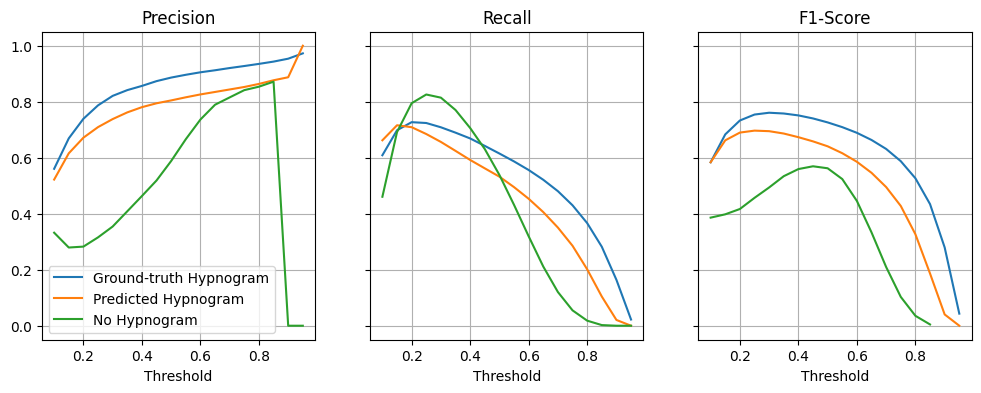
\includegraphics[width=\textwidth]{images/SleepStages}
    \caption{Precision, recall, and F1-score for the SDB detection model with different sleep stage information. The more the models sleep stage information gets to the ground-truth hypnogram, the better the performance.}
    \label{fig:sleep-stage-importance}
\end{figure}

\section{Correcting model output}

After applying the threshold for the prediction, a correction step was applied. This step removed events shorter than a specified number of seconds (called the correction size) and merged events that were closer than the correction size. Figure \ref{fig:correction-size} displays the impact of the correction size and shows that settings this value too low allows more prediction errors to pass through, while setting it too high removes many true positives. A correction size of 3 seconds seems to be the best option.

\begin{figure}
    \centering
    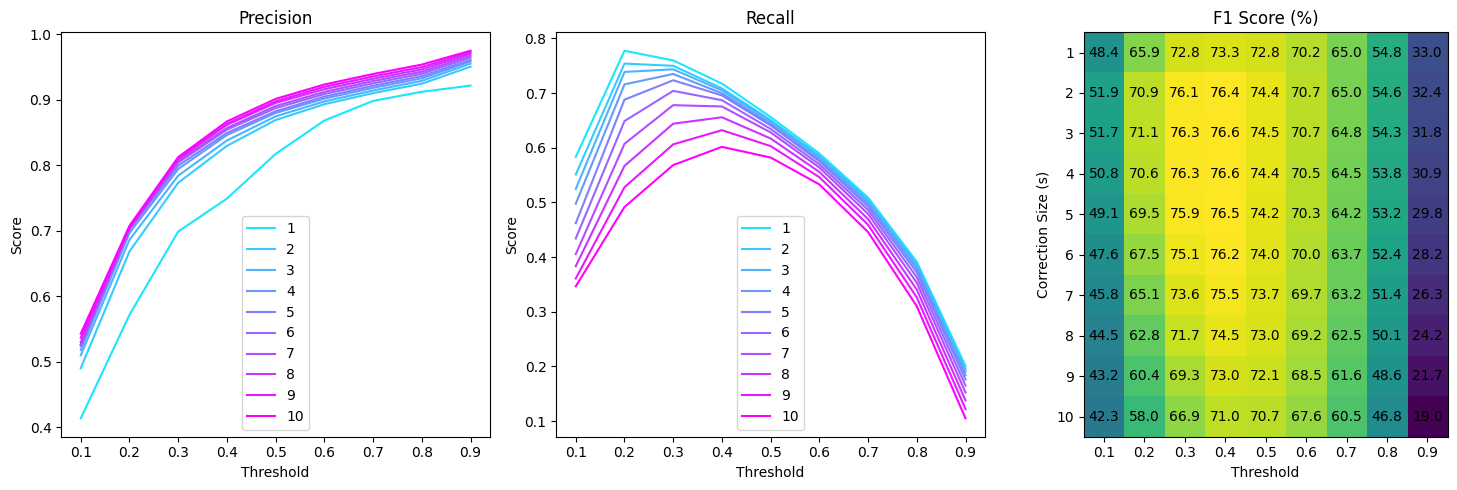
\includegraphics[width=\textwidth]{images/CorSizeMetrics}
    \caption{Event-level metrics for our SDB detection model for different correction sizes over the thresholds. As the precision grows with bigger correction sizes, the recall decreases. While most of both changes are somewhat evenly, there is a big difference in no correction (size of 1) to a small correction (of size 2) for the precision. Important to note is that, as with the preprocessing experiments, these results came from tests with the ground-truth hypnogram.}
    \label{fig:correction-size}
\end{figure}
